%*-------------------------------------------------------------------------*
%*                 Copyright 2013-2015 Core Physics, Inc.                  *
%*  Under terms of the contract to support CASL, there is a non-exclusive  *
%*  license for use of this work by or on behalf of the U.S. Government.   *
%*-------------------------------------------------------------------------*
%
% @version CVS $Id: assemblies.tex,v 1.23 2015/02/23 00:56:17 scott Exp $
%
%%%%%%%%%%%%%%%%%%%%%%%%%%%%%%%%%%%%%%%%%%%%%%%%%%%%%%%%%%%%%%%%
\section{Assembly Description}

The [ASSEMBLY] block contains the geometric description of a unique fuel assembly design (type).
Multiple [ASSEMBLY] blocks are allowed to describe different assembly designs in the core.

If there are multiple assembly designs that are geometrically identical (i.e. everything is the same except
the enrichments), then they can all be defined in a single [ASSEMBLY] block.
Each assembly type will have a unique {\it axial} card with possibly unique axial levels and lattice types.
Assemblies within a single reload typically have a design similar enough that they can share a single
[ASSEMBLY] block.

If assembly designs are not geometrically identical (e.g. different vendors, different generations, etc.)
they need to be defined in separate [ASSEMBLY] blocks.
One advantage to having separate blocks for each assembly design is that each design can be
modeled (and archived) independently without having to rely on global definitions.

A typical PWR assembly is shown in Figure~\ref{fig:assembly}.  Refer to this figure in the following discussions.
\begin{figure}
\begin{center}
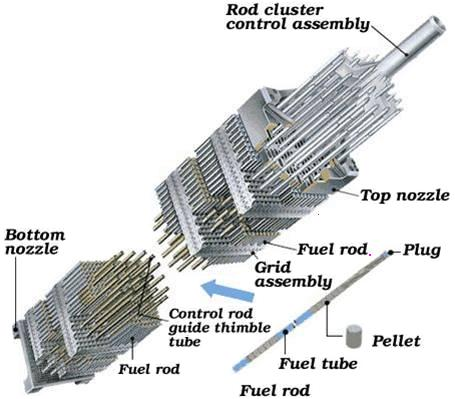
\includegraphics[width=4in]{figs/PWR-assembly.jpg}
\end{center}
\caption{\label{fig:assembly} PWR Fuel Assembly (source: Public internet).}
\end{figure}

A complete listing of all the input cards in the [ASSEMBLY] block is located in Section~\ref{sec:assemblycards}.

%%%%%%%%%%%%%%%%%%%%%%%%%%%
\subsection{Initial Data}

Each assembly block must contain a geometry description with the number of pins across the assembly and
the pin pitch.  An assembly block can also include an optional title card.
\begin{verbatim}
  title "Westinghouse 17x17"      ! assembly title
  npin 17                         ! number of pins across one side
  ppitch 1.260                    ! pin pitch (cm)
\end{verbatim}

The number of pins {\it npin} must be the same for every assembly in a core.

The inter-assembly gap on each side of the assembly is calculated as $[apitch-npin*ppitch]/2$

The fuel and structural materials are defined with the following cards.
See Chapter~\ref{chap:materials} for a complete description of the material inputs.
\begin{verbatim}
  fuel U31 10.257 95.0 / 3.1   ! mat, density (g/cc), Theoretical density (%)
                               !    / U-235 enrichment (%)
  mat inc   8.19               ! mat, density (g/cc)
  mat ss    8.0
  mat zirc4 6.56
\end{verbatim}

%%%%%%%%%%%%%%%%%%%%%%%%%%%
\subsection{Cell Descriptions}

Cell cards are used to describe ``pincells''.  A pincell is defined as a configuration
of concentric cylinders (or rings) centered in a square region of coolant.
Cell configurations can be used to model fuel rods or guide tubes,
as shown in Figure~\ref{fig:pincell}.
\begin{figure}
\begin{center}
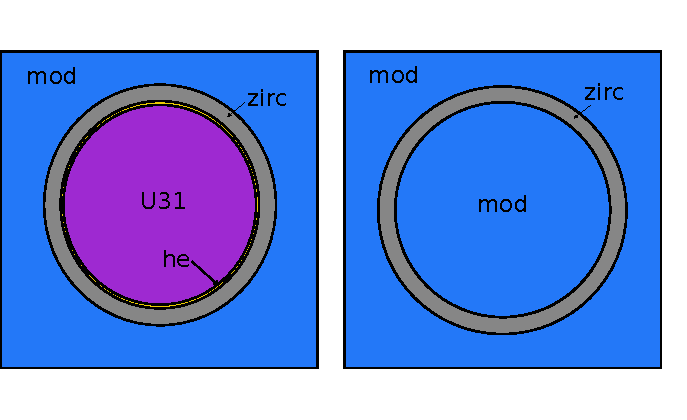
\includegraphics[width=4in]{figs/pincell1.pdf}
\end{center}
\caption{\label{fig:pincell} Pincell diagrams of a fuel rod and a guide tube.}
\end{figure}

The first parameter on the {\it cell} card is the cell ID.
This is followed by a list of radii for each ring in the cell, followed by a slash.
After the slash is a list of materials that compose each ring.
The cell ID's are used in the rod maps described in the next section.

\begin{verbatim}
  cell 1     0.4096 0.418 0.475 / U31 he zirc4
  cell GT           0.561 0.602 / mod    zirc4      ! guide tube
  cell IT           0.561 0.602 / mod    zirc4      ! instrument tube
  cell 7            0.418 0.475 / mod    mod        ! empty location
  cell 8            0.418 0.475 /     he zirc4      ! plenum
  cell 9                  0.475 /        zirc4      ! pincap
\end{verbatim}

In this example, in cell ``1'', the material ``U31'' extends from radius 0 to 0.4096.
The material ``he'' extends from a radius 0.4096 to 0.418.
The materials ``U31'' and ``he'' are defined on {\it fuel} and {\it mat} cards, respectively.
(Refer to Chapter~\ref{chap:materials} for a complete description on defining materials.)

The outside of each cell is automatically filled with the special material ``mod'', which
refers to the moderator (or coolant).
The composition of ``mod'' is calculated by the codes using the local T/H conditions and the
soluble boron concentration, and cannot be specified by a user on a {\it mat} card.

In the example above, the guide tube (GT) and instrument tube (IT) descriptions
use the special moderator material ``mod'' to define the moderator material on both
the inside and outside of the tubes.

Note that large water rods that span more than one lattice cell are not currently supported in the input
(e.g. large CE water rods that span four lattice cells).
In the future, an option will be added to the {\it cell} card to specify if a water rod spans more than one cell. 

%%%%%%%%%%%%%%%%%%%%%%%%%%%
\subsection{Lattice Descriptions}

Once the cells are defined, they are placed into 2D ``lattices'' as shown below.
Like the core maps, the lattice maps can be entered with either full-symmetry, qtr-symmetry,
or octant-symmetry.  The maps below are octant symmetric maps for 17x17 assembly designs.
\vfill   % don't split map
\begin{verbatim}
  rodmap FUEL1
      IT
       1 1
       1 1 1
      GT 1 1 GT
       1 1 1  1 1
       1 1 1  1 1 GT
      GT 1 1 GT 1  1 1
       1 1 1  1 1  1 1 1
       1 1 1  1 1  1 1 1 1

  rodmap LGAP1
      IT
       7 7
       7 7 7
      GT 7 7 GT
       7 7 7  7 7
       7 7 7  7 7 GT
      GT 7 7 GT 7  7 7
       7 7 7  7 7  7 7 7
       7 7 7  7 7  7 7 7 7

  rodmap PLEN1
      IT
       8 8
       8 8 8
      GT 8 8 GT
       8 8 8  8 8
       8 8 8  8 8 GT
      GT 8 8 GT 8  8 8
       8 8 8  8 8  8 8 8
       8 8 8  8 8  8 8 8 8

  rodmap PCAP1
      IT
       9 9
       9 9 9
      GT 9 9 GT
       9 9 9  9 9
       9 9 9  9 9 GT
      GT 9 9 GT 9  9 9
       9 9 9  9 9  9 9 9
       9 9 9  9 9  9 9 9 9
\end{verbatim}

Rod maps define each unique axial level in the assembly.
The first parameter is the lattice name (e.g. FUEL1, PCAP1, etc.),
followed by a map of the {\it cell} ID's.

Each entry in a rod map must be a valid cell ID.

%%%%%%%%%%%%%%%%%%%%%%%%%%%
\subsection{Axial Descriptions}

After rod maps are defined for each axial level, the lattices are ``stacked'' into
an assembly using an {\it axial} card as shown below.

\begin{verbatim}
  axial A1    6.050
      LGAP1  10.281
      PCAP1  11.951
      FUEL1 377.711
      PLEN1 393.711
      PCAP1 395.381
      LGAP1 397.501
\end{verbatim}

The {\it axial} card tells the code how to place the lattices axially.
The first parameter is the name of the assembly (A1), followed by a
list of elevations and lattice types.
For example, lattice ``FUEL1'' extends from 11.951 to 377.711 cm axially.

Multiple assembly types can be defined in a single [ASSEMBLY] block by using
multiple {\it axial} cards, each with a unique assembly ID.

All axial elevations are defined relative to the top of the lower core plate.

%%%%%%%%%%%%%%%%%%%%%%%%%%%
\subsection{Grid Spacer Descriptions}

Grid cards are used to define unique grid spacer types.
The following example defines two grid types, ``END'' and ``MID''.
\begin{verbatim}
  grid END inc   1017  3.866   ! grid spacer material, mass(g), height(cm)
  grid MID zirc4  875  3.810
\end{verbatim}

The grid types are placed axially with the {\it grid\_axial} card:
\vfill   % don't split map
\begin{verbatim}
  grid_axial
      END  13.884
      MID  75.2
      MID 127.4
      MID 179.6
      MID 231.8
      MID 284.0
      MID 336.2
      END 388.2
\end{verbatim}

The elevations are the midpoints of the spacer grid and are relative to the top of the lower core plate.

%%%%%%%%%%%%%%%%%%%%%%%%%%%
\subsection{Nozzle Descriptions}

The assembly nozzles are modeled in the neutronics codes as smeared materials.  This is a very good
approximation since the nozzles are not in the active fuel region and are mostly
composed of water, steel, and zirconium.  The user only specifies a nozzle mass and a nozzle height.
The total volume of the nozzle region is calculated from the assembly pitch and nozzle height.
The volume of the nozzle is calculated from the nozzle mass and density.
The volume of the coolant is then calculated as the total volume minus the volume of the nozzle.
The coolant density is updated with the local T/H conditions.

% A typical PWR assembly nozzle is shown in Figure~\ref{fig:nozzle}.
% \begin{figure}
% \begin{center}
% 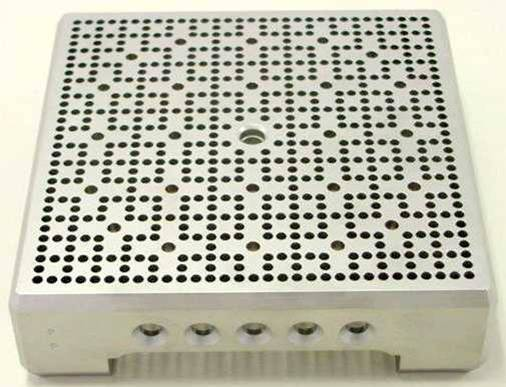
\includegraphics[width=4in]{figs/nozzle.jpg}
% \end{center}
% \caption{\label{fig:nozzle} PWR Assembly Lower Nozzle.}
% \end{figure}

\begin{verbatim}
  lower_nozzle  ss 6.05  6250.0  ! mat, height (cm), mass (g)
  upper_nozzle  ss 8.827 6250.0  ! mat, height (cm), mass (g)
\end{verbatim}

Only a single material can be specified on a nozzle card.  If the user wants to use
more than one material to define a nozzle, they can define a custom material that
is a mixture of the materials and then use the custom material in the nozzle card.

Note that the {\it lower\_nozzle} height should match the bottom elevation on the {\it axial} card.
The {\it upper\_nozzle} height + the top elevation on the {\it axial} card must match the
core {\it height} in the [CORE] block.
The input parser does not currently perform a check to make sure the elevations are consistent.
Therefore, this check should be performed in each of the individual physics codes.

%%%%%%%%%%%%%%%%%%%%%%%%%%%%%%%%%%%%%%%%%%%%%%%%%%%%%%%%%%%
\section{Control Rod Assembly Description}

The [CONTROL] block contains the geometric description of a control assembly.

A control rod assembly is defined in the same way that a fuel assembly is defined.
The user specifies cells, lattices, and axial descriptions of the control rod assembly. 
The main difference between the control rod assembly and the fuel assembly is that
the control rod assembly describes what is inside the guide tubes and the fuel assembly
defines the guide tubes themselves.

Control rod positions change during operation, so the geometric description of a control rod
should always be for a rod in the {\bf fully inserted} position.
In the example below, the bottom of the control rod in the fully inserted position is 
at an axial location of 15.46 cm.

\begin{verbatim}
  title "B4C control rods with AIC tips" 
  npin 17

  cell 1  0.382 0.386 0.484 / aic he ss      ! AIC cell
  cell 2  0.373 0.386 0.484 / b4c he ss      ! B4C cell

  rodmap  AIC
     -
     - -
     - - -
     1 - - 1
     - - - - -
     - - - - - 1
     1 - - 1 - - -
     - - - - - - - -
     - - - - - - - - -

  rodmap  B4C
     -
     - -
     - - -
     2 - - 2
     - - - - -
     - - - - - 2
     2 - - 2 - - -
     - - - - - - - -
     - - - - - - - - -

  axial CR1 15.46 AIC  376.44 B4C  394.3
\end{verbatim}

The name of the control rod ``CR1'' refers to the control rod type in the
{\it crd\_map} in the [CORE] block.

Control rods positions are assigned to a control rod bank with the {\it crd\_bank} map
in the [CORE] block, and then the banks are positioned with the 
{\it rodbank} card in the [STATE] block.

Note that the locations of the control rod fingers must match the guide tube locations in the
corresponding [ASSEMBLY] block descriptions.  Furthermore, the outer radii of the control
rod fingers must be smaller than the inner radii of the guide tubes.
The input parser does not currently perform a check to make sure the control rod finger
descriptions are consistent with the guide tube descriptions.
This check should be performed in each of the individual physics codes.

The user can define materials in the [CONTROL] block.  These materials only have scope in
this block and are not accessible by other blocks.  See Chapter~\ref{chap:materials} for details.

A complete listing of all the input cards in the [CONTROL] block is located in Section~\ref{sec:controlcards}.

%%%%%%%%%%%%%%%%%%%%%%%%%%%
\subsection{Control Rod Stroke}
\label{sec:stroke}

The difference between control rod descriptions and assembly descriptions is that
the control rods move during operation.  This movement is defined with a {\it stroke} card.

The first value on the {\it stroke} card is the total length of the control rod travel (stroke)
from fully inserted to fully withdrawn.

The second value on the {\it stroke} card is the number of steps in the fully withdrawn position.
Step 0 is the fully inserted position.  The number of steps in the fully withdrawn position 
is specified by the user, but 228 steps is often used for typical Westinghouse PWR's.
\begin{verbatim}
  stroke  360.0 228      ! stroke (cm), number of steps fully withdrawn
\end{verbatim}

To position the control rods in percent withdrawn (\%), the number of steps should be set to 100 and
each step will signify 1\% withdrawn.

The geometry description in the input is for a control rod in the fully inserted position (step 0).

\subsection{Control Rod Position Example}

From the {\it axial} card shown above, the bottom of the AIC at the fully-inserted position is 15.46 cm.
From the {\it stroke} card, the total stroke is 360.0 cm and the number of steps in the fully withdrawn
position is 228 steps.
Therefore, the bottom elevation of the AIC lattice at step N will be
\begin{equation}
   E(N) = 15.46 + \frac{360.0 \cdot N}{228}
\end{equation}

Using this formula, the bottom elevation of the AIC lattice at the following step positions is:
\begin{itemize}   % itemize = bullet list
 \item step 228 (fully withdrawn)= 15.46 + 360.0 * 228 / 228 = 375.46 cm
 \item step 100 = 15.46 + 360.0 * 100 / 228 = 173.35 cm
 \item step 0 (fully inserted) = 15.46 + 360.0 * 0 / 228 = 15.46 cm
\end{itemize}

%%%%%%%%%%%%%%%%%%%%%%%%%%%%%%%%%%%%%%
\section{Insert Description}
An assembly insert is defined in the same way as a fuel assembly or control rod assembly is defined.
The user defines the insert using cells, lattices, and axial descriptions.

The fuel assembly description should contain the guide tube descriptions and the insert description
defines what is inserted in the guide tubes.  Assembly inserts can be inserted and withdrawn
during a core shuffle (by specifying a {\it insert\_map} card in the [CORE] block),
but cannot be moved during a cycle depletion.

The insert and control rod descriptions are very similar, with the only difference being that the
insert cannot change position axially during a cycle depletion and a control rod moves axially
during operations.

The following example shows a definition of a Pyrex insert.

\begin{verbatim}
[INSERT]
    title "Pyrex"
    npin 17
    mat pyrx1 2.25 pyrex-vera
    cell 1  0.214 0.231 0.241 0.427 0.437 0.484 / he ss he pyrx1 he ss
    rodmap  PY24
       -
       - -
       - - -
       1 - - 1
       - - - - -
       - - - - - 1
       1 - - 1 - - -
       - - - - - - - -
       - - - - - - - - -

    axial INS24  15.76 PY24 376.441
\end{verbatim}

The name of the insert ``INS24'' refers to an insert type defined in the
{\it insert\_map} in the [CORE] block.

The locations of the insert fingers must match the guide tube locations in the
corresponding [ASSEMBLY] block descriptions.  In addition, the outer radii of the insert
fingers must be smaller than the inner radii of the guide tubes.
The input parser does not currently perform a check to make sure the insert finger
descriptions are consistent with the guide tube descriptions.
This check should be performed in each of the individual physics codes.

As with [ASSEMBLY] blocks, multiple insert types can be defined in a single [INSERT]
block by using multiple {\it axial} cards, each with a unique insert ID.

A complete listing of all the input cards in the [INSERT] block is located in Section~\ref{sec:insertcards}.

%%%%%%%%%%%%%%%%%%%%%%%%%%%%%%%%%%%%%%
\section{Detector Description}
A detector string is defined in the same way that a fuel assembly or insert assembly is defined.
The user defines cells, lattices, and axial descriptions for the detector string.

The insert and detector descriptions are very similar, with the difference being that
detectors have special properties used to calculate instrumentation signals.

\begin{verbatim}
  [DETECTOR]
    title "Incore instrument thimble"
    npin 17

    mat he 0.0001786
    mat ss 8.0

    cell 1  0.258 0.382 / he ss

    rodmap  LAT
       1
       - -
       - - -
       - - - -
       - - - - -
       - - - - - -
       - - - - - - -
       - - - - - - - -
       - - - - - - - - -

    axial D1  0.0 LAT 406.337
\end{verbatim}

The name of the detector ``D1'' refers to a detector type defined in the
{\it det\_map} in the [CORE] block.

A complete listing of all the input cards in the [DETECTOR] block is located in Section~\ref{sec:detectorcards}.



